\section{DDlog Implementation}\label{sec-system}

\subsection{Compiling DDlog to Differential Dataflow}

\paragraph{Differential Dataflow.}
The core execution engine of DDlog is Differential Dataflow (DD).
Differential Dataflow~\cite{differential-dataflow-paper} is a
streaming big-data processing system which provides incremental
(differential) computation.  DD is an \emph{incremental}
map-reduce-like system, but supporting a wide set of relational
operators, including recursion (fixed-point) and joins.  Section 4.3
in~\cite{differential-dataflow-paper} describes the core relational
operators that are used by our compiler to implement DDlog operators.
DD is described in several
publications~\cite{timely-dataflow,differential-dataflow-paper} and
has an open-source implementation with online
documentation~\cite{dd-mdbook,dd-reference}.

\paragraph{Compilation.}
Figure~\ref{fig:compiler-flow} shows how DDlog programs are compiled.
The DDlog compiler is written in Haskell.  The compiler generates Rust
code (as text files); the Rust code is compiled and linked with the
open-source Rust version of the DD
library~\cite{differential-dataflow}.  The DD engine operates on
multisets, where elements can have positive or negative cardinalities;
to get a set semantics we need to apply \texttt{distinct} operators on
some multisets, in particular, output collections.

The DDLog compiler performs parsing, type inference, validation, and
several optimization steps.  In order to compute incremental results
the DD runtime has to maintain temporal indexes (indexed by logical
time), containing previous versions of relations.  Many of our
optimizations are geared towards reducing memory consumption; for
example, we attempt to share indexes between multiple collections and
operators.  We use reference counting for large values, but
stack-based implementations for small values.  The non-linear
operators (like \texttt{distinct}) can be very expensive, so we try to
minimize their usage.  The compiler attempts reuse common prefixes of
disjoint rules.

\begin{figure}
\begin{center}
    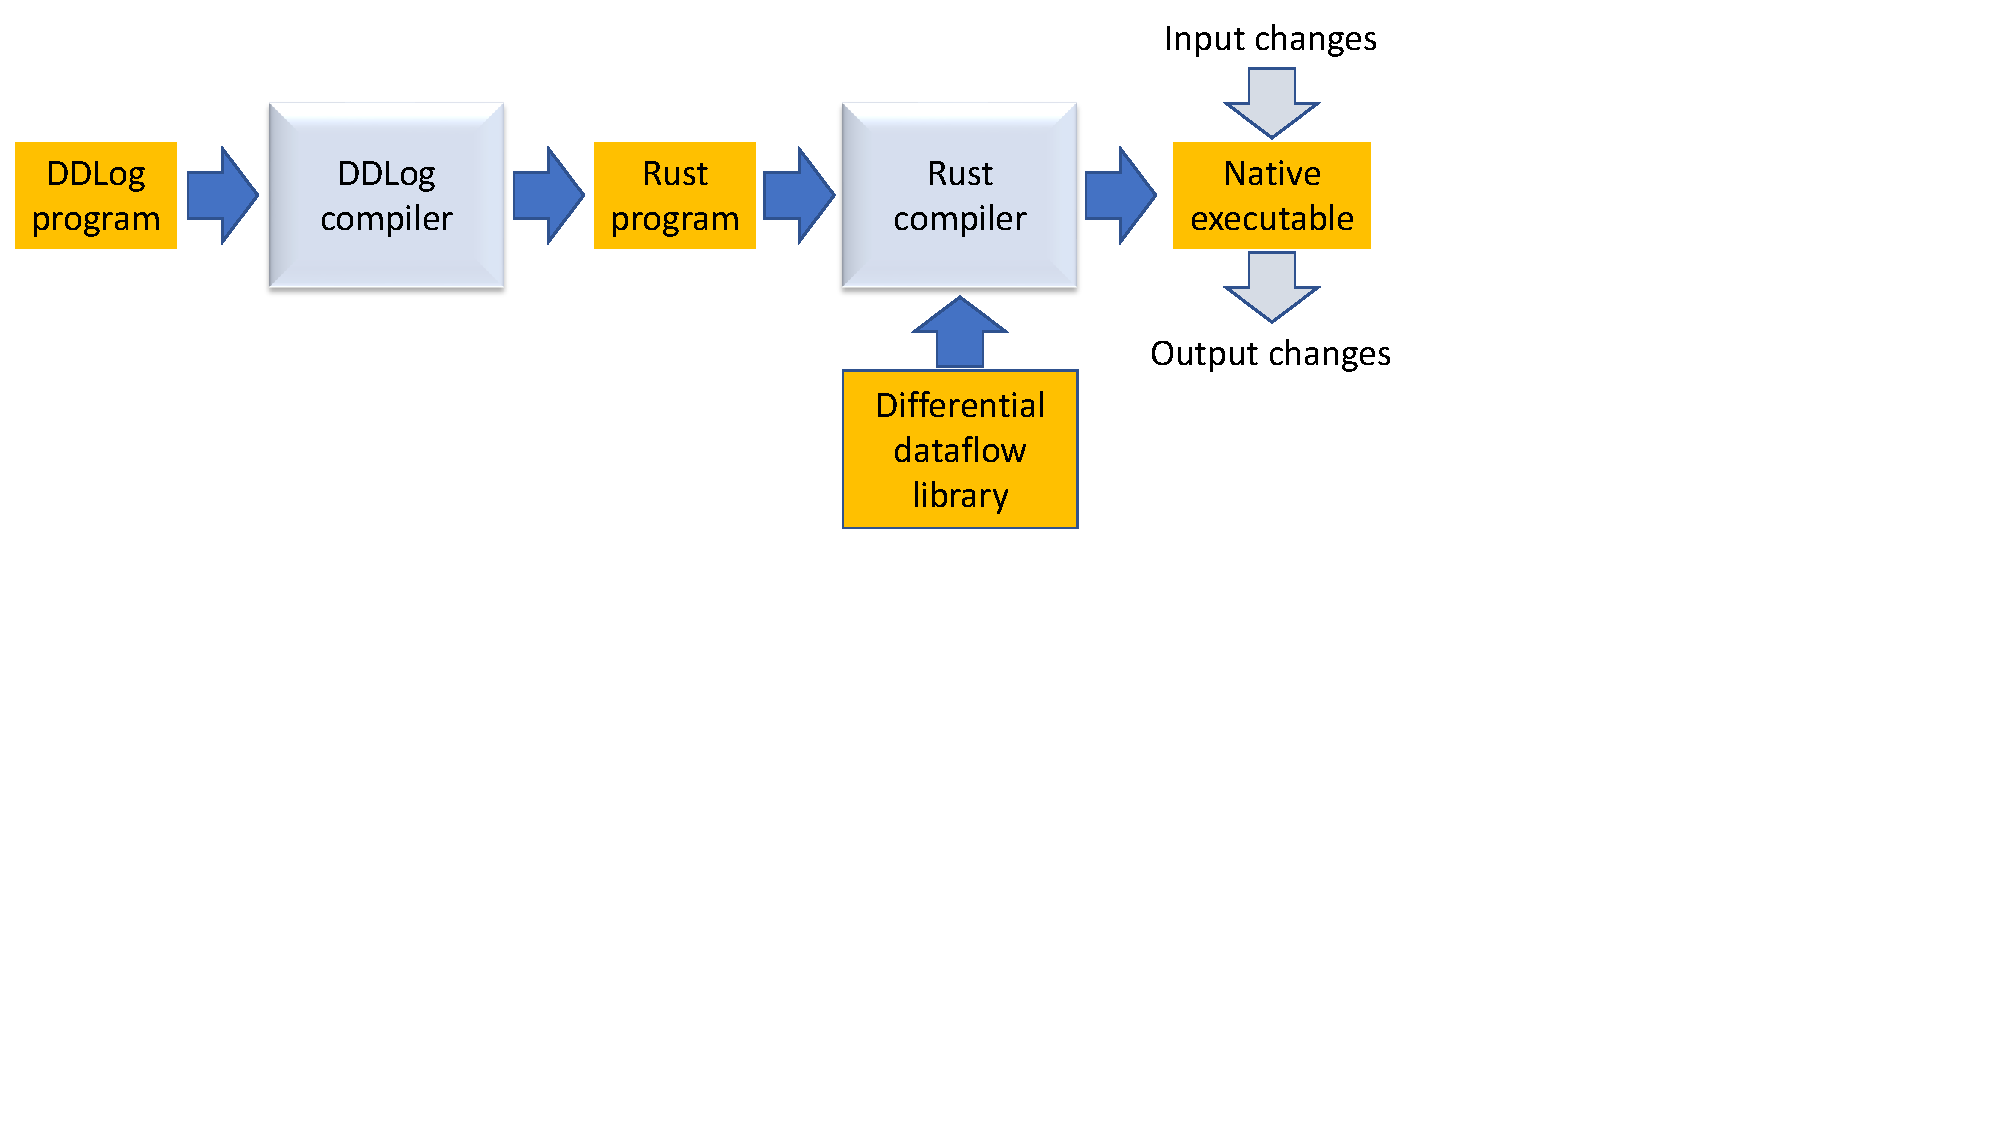
\includegraphics[width=.6\columnwidth,clip=true,trim=0in 4in 4in
      0in]{compiler-flow.pdf}
\end{center}
    \caption{DDlog compilation flow.\label{fig:compiler-flow}}
\end{figure}

The output of the DDlog compiler is a dataflow graph, which may
contain cycles (introduced by recursion).  The nodes of the graph
represent relations; the relations are computed by dataflow relational
operators.  Edges connect each operator to its input and output
relations.  DD natively implements the following operators: map,
filter, distinct, join, antijoin, groupby, union, aggregation, and
flatmap.  Each operator has a highly optimized implementation,
incorporating temporal indexes that track updates to each relation
over time and allow efficient incremental evaluation.  The DD library
is responsible for executing the emitted dataflow graph across many
cores by running a user-defined number of worker threads.

\subsection{Interacting with DDlog programs}

\paragraph{Transactional API.}
The interaction with a running DDlog program is done through a
transactional API.  At any time only one transaction can be
outstanding.  After starting a transaction the user can insert and
delete any number of tuples from input relations.  When attempting to
commit a transaction all updates are applied atomically and changes to
all output relations are produced.  Users register an upcall to be
notified of these changes.

The DDlog API is implemented in Rust, with bindings available for
other languages, currently C and Java.

\paragraph{The command-line interface.}
For every DDlog program the compiler generates a library that exports
the transactional API, which can be invoked from Rust or other
languages.  The compiler also generates a command-line interface
program (CLI) that allows users to interact with the DDlog program
directly via a command line or a script.  The CLI allows users to
start transactions, insert or delete tuples in input relations, commit
transactions, dump the contents of relations, and get statistics about
resource consumption.  The CLI is also used for regression testing and
debugging.

%% \paragraph{C and Java interfaces}
%% The DDlog API is natively
%% implemented in Rust, with bindings available for other languages,
%% currently C and Java.
%%
%% We illustrate the Java API to a simple DDlog program with a
%% skeleton example in Figure~\ref{fig:javaapi}.

%% \begin{figure}
%%   \footnotesize
%%   \begin{lstlisting}[language=ddlog]
%% // DDlog program
%% input relation Parent(parent: string, child: string)
%% output relation Ancestor(ancestor: string, descendant: string)
%% Ancestor(ancestor, descendant) :- Parent(ancestor, descendant).
%% Ancestor(ancestor, descendant) :- Ancestor(ancestor0, ancestor1),
%%                                   Parent(ancestor1, descendant).
%%   \end{lstlisting}

%%   \begin{lstlisting}[language=Java]
%% // Java program interfacing with DDlog program
%% static class Parent {
%%   String parent;
%%   String child; }
%% static class Ancestor {
%%   String ancestor;
%%   String descendant; }

%% /* Instantiate the DDlog program; add a record to the
%%  * Parent relation. */
%% static void main() {
%%   DDlogAPI api = new DDlogAPI(2 /* threads */,
%%                r -> onCommit(r) /* callback */);
%%   int parentRelation = api.getTable("Parent");
%%   Parent p = new Parent();
%%   p.parent = "Mike"; p.child  = "John";
%%   /* Create DDlog insert command. */
%%   DDlogCommand command = new DDlogCommand(
%%      DDlogCommand.Kind.Insert, parentRelation, p);
%%   int exitcode = api.start();  // start transaction
%%   DDlogCommand[] commands = new DDlogCommands[1];
%%   commands[0] = command;
%%   exitcode = api.applyUpdates(commands);
%%   /* commit transaction; causes the callback to be
%%    * invoked for each new or deleted output record.
%%    * commit blocks until all upcalls have been invoked. */
%%   exitcode = api.commit();
%%   api.stop();
%% }

%% /* Callback invoked on commit once for each insertion or
%%  * deletion in an output relation. */
%% static void onCommit(DDlogCommand command) {
%%   int outputRelation = command.tableId;
%%   Ancestor value = command.getObject<Ancestor>();
%%   if (command.kind == DDlogCommand.Kind.Insert)
%%     // ancestor inserted
%%   else
%%     // ancestor deleted
%% }
%% \end{lstlisting}
%% \caption{Example program showing the Java API to pass and receive data
%%   from a DDlog program.\label{fig:javaapi}}
%% \end{figure}
